In order to test the AI, an application will be developped.
This application will include a two-player mode, a one-player mode and a demonstration mode (AI versus AI).
In the case where several AI have been implemented, the user will be able to choose which one to play against.

\begin{figure}[!h]
\centering
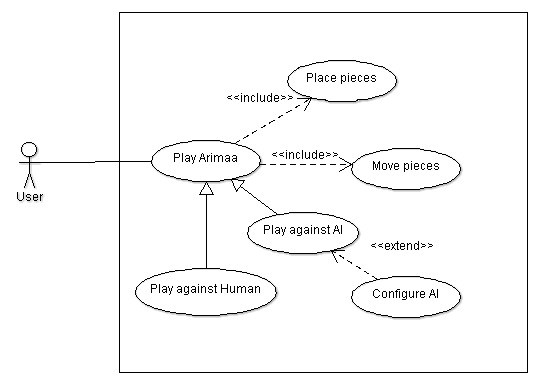
\includegraphics[width=0.7\textwidth]{2General_Architecture/2.1Behaviour_of_the_Game/Pictures/Application_UCD}
\caption{The user-case diagram describing the application}
\label{fig:pieces}
\end{figure}

In order to make the game easy to play, this application will provide a graphical uer interface (further referred to as \emph{UI}). % as described in part ??
This UI, as well as the algorithm for the AI, will act upon the game model, so as to inform it of what moves were made.
The UI will also regularly update to give the player feedback on the progression of the game.